%%Aquí se describe el estado del arté, o bien el marco teórico.

\section{Introducción.}


\section{Conceptos preliminares de óptica.}
    
    {\bfseries\Large Añadir una introducción a la sección.}
    
% Presentar el modelo de camara pinhole
\subsection{El modelo pin-hole\label{sec:pin-hole}}
    También llamado \emph{perspectiva pinhole} o bien \emph{perspectiva central}, se trata de un modelo propuesto por Brunelleschi al incio del siglo XV, su propósito se basa en la formación de imágenes a partir de los rayos provenientes de una fuente de luz que a su vez, estos atraviesan un orificio ubicado en el lado de una caja y en su lado opuesto se encuentra un plano traslúcido donde los rayos son reflejados de manera invertida. El modelo de perspectiva pinhole fue uno de los primeros modelos para formación de imágenes, resulta ser simple pero no estríctamente aplicable. \citet{Forsyth2003}
    
    En la figura \ref{perspectivaPinhole} se muestra un ejemplo de como se forman las imágenes en el modelo de perspectiva pinhole, basado en ello y en la óptica se generan las ecuaciones:
    
    \begin{equation}
         \begin{array}{ll}
         x'= f' x/z ;\\
         y'= f' y/z \end{array}.
    \end{equation}
   
    

    \begin{figure}[ht]
        \centering
        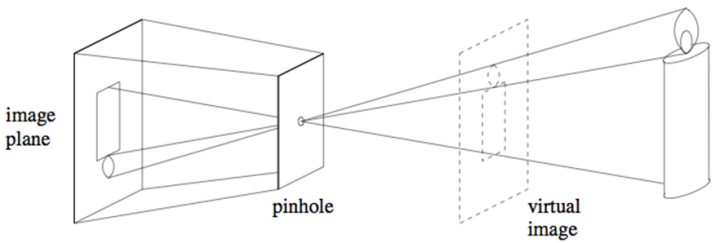
\includegraphics[scale=1.25]{GraficosEdArt/fig1.png} 
        \caption{Modelo de perspectiva pinhole. \citet{Forsyth2003}}
        \label{perspectivaPinhole}
    \end{figure}
    

\subsection{El modelo de lente delgado}
% Presentar el modela de la cámara de lente delgado.
Consta de dos superficies esféricas y con un índice de refracción de uno, de allí el término de "delgado" (ya que el rayo que incide en un extremo, es refractado en el otro extremo de manera inmediata).
El modelo geométrico que lo representa se muestra en la figura \ref{lenteDelgado}, los rayos provenientes del punto P atraviesan el lente de tal forma que los rayos que pasan por el punto $O$ no son refractados. \citet{Forsyth2003}

    \begin{figure}[ht]
        \centering
        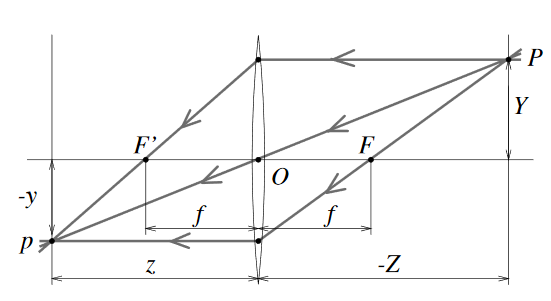
\includegraphics[scale=.75]{GraficosEdArt/ModeloLenteDelgado.PNG} 
        \caption{Un lente delgado. Los rayos pasan a través del punto $O$ no son refractados. Los rayos paralelos al lente óptico son enfocados al punto focal $F'$. \citet{Forsyth2003}}
        \label{lenteDelgado}
    \end{figure}
El modelo algebráico que define a un lente delgado se muestra en la ecuación \ref{eqn:lensthin} , que relaciona la profundidad del punto de objeto $z$, la profundidad del punto de imagen $z'$ y una distancia focal $f$.

\begin{equation} \label{eqn:lensthin}
\large  \frac{1}{z'} - \frac{1}{z} = \frac{1}{f}
\end{equation}


\subsection{El diafragma}
    El diafragma en un sistema de lentes, es una entrada circular, en el cual la luz viaja a través de ella, también es llamado paraderos, porque frenan el paso de luz en algunas regiones. Si limitan el campo de visión de un instrumento son llamados paraderos de campo, en otros casos actuan como paraderos de apertura, reduciendo la cantidad de luz que pasa através del sistema. \citet{paschotta_2020}
\subsection{La apertura}
    La apertura en óptica es el máximo diametro de luz que puede atravesar un sistema óptico. Es limitado por el tamaño que sostiene el componente óptico, o el tamaño del diafragma colocado en el conjunto de rayos de luz.\citep{encyclopediabritannica}
\subsection{La profundidad de campo}
    La profundidad de campo (DoF por sus siglas del inglés Depth of Fiel) es el rango en frente o dentrás del punto de enfoque, donde los objetos permanecen enfocados. Cuanto más abierto es el tamaño de apertura (Número-f inferior), la profundidad de campo disminuye. La profundidad de campo juega un papel importante en la parte de ver y sentir de una imagen. \citep{canon_australia_2019}
\subsection{Función de dispersión de punto}
    La función de dispersión de punto ideal es la difracción en tres dimensiones de los patrones de luz emitidos desde un punto de fuente de luz infinitamente pequeño en el especimen y es transmitido al plano de imagen a través de una apertura numérica alta objetiva. Este es considerado la unidad fundamental de una imagen en modelos teóricos basados en su formación. Cuando la luz es emitida desde algún objeto punto, una fracción de esta es recolectada por el objetivo y enfocada en el punto correspondiente en la imagen del plano. Sin embargo, los objetivos del lente no enfocados a la luz emitida a un punto infinitamente pequeño en el plano de imagen. Más bien, las ondas de luz convergen e interfiere en el punto focal para producir un patrón de difracción de anillos concéntricos de luz rodeando un central, disco brillante, cuando es visto en el plano x-y. El radio del disco es determinado por la apertura numérica, entonces la potencia de resolución de un lente objetivo puede ser evauluado por medir el tamaño del \emph{disco Airy} (llamado así por George Biddel Airy). La imagen del patrón de difracción puede ser representado como una distribución de intensidad, mostrada en la figura \ref{psfDemo}. La porción de brillo central del disco Airy y los anillos concéntricos de luz corresponden a los picos de intensidad en la distribución. En la figura \ref{psfDemo}, la intensidad relativa es graficada como una función de posición espacial para PFS's desde objetivos con una apertura numérica de 0.3 y 1.3. El ancho máximo en la mitad del máximo es indicado para el valor más pequeño de la alta apertura numérica objetiva junto al límite Rayleigh. \citep{ruttenfusser_wilson_davidson}.

\subsection{Perspectiva de proyección}

\subsection{Homografía}    
    
\begin{figure}[ht]
    \centering
    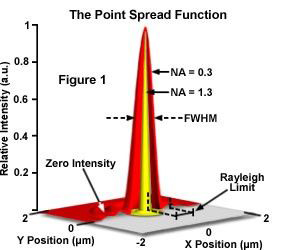
\includegraphics[scale=1]{GraficosEdArt/psfintrofigure1.jpg} 
    \caption{Ejemplo de función de dispersión de punto.\citep{ruttenfusser_wilson_davidson}}
    \label{psfDemo}
\end{figure}
        
\section{Antecedentes}
    Para poder llevar a cabo este trabajo de investigación se realizó una exploración de la literatura referente a la profundidad de campo, en la búsqueda de una métrica para poder realizar el segmentado de partes enfocadas en una imagen de un canal de luminosidad, con la finalidad de generar el modelo deseado.

    En \citet{Pentland} se menciona un modelo para poder estimar la profundidad de campo a partir de la cantidad de desenfoque en una región, dicho modelo contiene parámetros que son conocidos, como lo es el tamaño del lente, la cantidad de desenfoque y la distancia al plano de la imagen. A continuación se presenta el modelo descrito en el artículo:\\
\\
\begin{equation} \label{eqn:model1}
\large D = \frac{F v_{0}}{v_{0} - F - \sigma f}
\end{equation}
\\
En la ecuación  \ref{eqn:model1} se presentan los parámetros anteriormente mencionados, donde $f$ es el número f del sistema de lentes, $F$ el tamaño del lente focal, $v_{0}$ la distancia al plano de la imagen y por último $\sigma$ que representa la cantidad de borrosidad o bien desenfoque, en una región determinada.
\\
Dicho modelo resulta ser de mucha utilidad, ya que puede ser usado como una métrica al momento de estar midiendo la cantidad de desenfoque en una imagen, con respecto al microscopio.

\begin{figure}[ht]
\centering
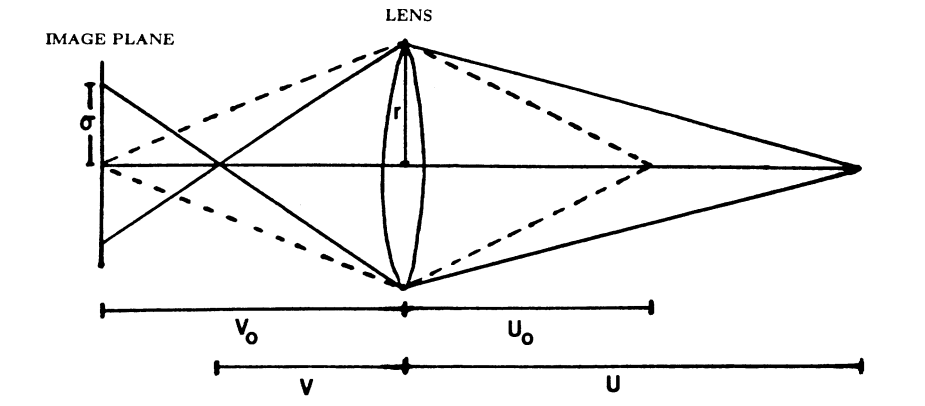
\includegraphics[scale=0.50]{GraficosEdArt/profcamp.PNG} 
\caption{Geometría de la imagen.\citet{Pentland}}
\label{fig1}
\end{figure}
En la figura \ref{fig1} se muestra el modelo de lente delgado, donde $U$ representa la distancia con respecto a la escena, lo cual,  genera una borrosidad, es decir, se genera un desfasamiento $\sigma$ en el plano de la imagen, dicho valor representa la cantidad de desenfoque y por otro lado la distancia $u_{0}$ representa el punto donde se genera un enfoque perfecto.
\\
\\
La idea principal se basa en medir el campo de profundidad en una imagen, nombrado como el gradiente de enfoque, dicho gradiente representa una distancia cuyo cálculo se lleva a cabo con la cantidad de desenfoque en una región, entonces, para ello se proponen dos métodos: la estimación de la cantidad de desenfoque a partir de discontinuidades agudas y la estimación a partir del cambio de apertura del lente, lo cual este no se acopla a los requerimientos del microscopio donde la apertura del lente se mantiene fija, por lo tanto no se abordará en este trabajo de investigación.
\\
\\
El método que se basa en el uso de discontinuidades agudas, cuya estimación de la $\sigma$ se obtiene a partir de los bordes obtenidos por una transformación de Laplace cuyas entradas serán la convolución entre la imagen original y una función de dispersión, lo cual se modela como un filtro de Gaussiano con una constante espacial $\sigma$, aplicando métodos de regresión lineal, sustituciones y despejes se obtiene la estimación del valor $\sigma$. 
\begin{figure}[ht]
\centering
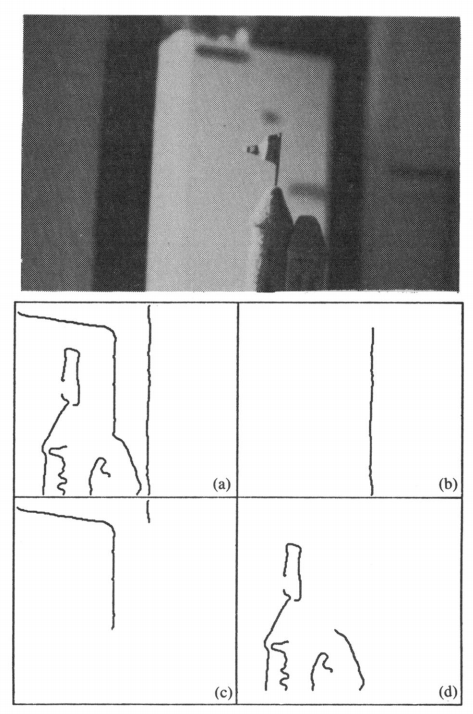
\includegraphics[scale=0.50]{GraficosEdArt/EvaluacionUSE.PNG} 
\caption{Evaluación del método estimación de desenfoque a partir del de discontinuidades agudas \citet{Pentland}}
\label{fig2}
\end{figure}
\\
\\
En la figura \ref{fig2} se muestra una imagen con un castillo de arena, un refrigerador y una puerta, dicha imagen fue evaluada en el método propuesto por \citet{Pentland}, los resultados de la evaluación se muestran en los cuadros con bordes en su interior, en el cuadro (a) se muestran todas las discontinuidades encontradas, mientras que en los otros cuadros (b), (c) y (d) se muestran los contornos que fueron segmentados de acuerdo a los valores de la distancia obtenida en la profundidad de campo.
\\
\\
La finalidad de llevar a cabo este método en el presente trabajo de investigación recae en la necesidad de segmentar las partículas de polen que se encuentran enfocadas bajo ciertos desplazamientos de la platina, a través de los contornos.
Entre la mayoría de los trabajos que se han realizado, van dirigidos hacia la búsqueda de un método cuyo objetivo se basa en la estimación del valor óptimo de enfoque que en algunos casos se puede tratar de la distancia al objeto o bien una distancia focal, todo dependiendo del hardware. Por otra parte la forma de modelar la borrosidad en una imagen es a partir de modificar la apertura de la cámara y en otros se genera a partir de una función de dispersión que lo modela, en este trabajo de investigación se explorarán ambas alternativas ya que la importancia radica más en el método para estimar la profundidad de campo.

En \citet{Mo2012} el autor propone un algoritmo basado en el umbral y en el gradiente máximo de una imagen, en el artículo se hace la comparación entre diferentes métodos que hacen uso de una función de gradiente, dicha función trabaja directamente con las componentes de altas frecuencias, de tal forma que si tenemos una imagen perfectamente enfocada, implica que predominan las altas frecuencias, por lo tanto la imagen se encuentra saturada de bordes. Por otra parte si se tiene una imagen fuera de enfoque o borrosa, entonces las altas frecuencias son atenuadas y por lo tanto la imagen se encuentra escasa de bordes.

La función de gradiente trabaja como un evaluador del comportamiento previamente descrito, de tal forma que evalua la claridad de la imagen. Entre algunas funciones conocidas se encuentra la función gradiente de Energía, de Roberts, de Tenengrad, de Brenner y la de varianza.
\\
El artículo propone una función de gradiente basada en la convolución de la imagen con cuatro máscaras de tipo Sobel, que representan el gradiente en dirección horizontal, vertical, diagonal positiva y diagonal negativa. A esta función se le etiqueta con el nombre de función de gradiente máximo $G(x,y)$.

La metodología de este trabajo de investigación consta de cuatro etapas, en la primera etapa se hace uso del algoritmo de Otsu para poder hallar el umbral óptimo $T_k$  y el factor de umbral $\alpha$ de tal forma que se obtiene el umbral global $T$ de la imagen.
%%Insertar calculo para el umbral global T.

En la segunda etapa se lleva a cabo el cálculo de una matriz integrada por las varianzas $\sigma^2(x,y)$ , obtenidas a partir de un conjunto de pixeles extraídos directamente de la imagen por una matríz ventana de 3 X 3 , de tal forma que se obtienen $(M-2)$X$(N-2)$ matrices de ventana, donde $M$ y $N$ son las dimensiones de la imagen. 
%Insertar equaciones de la varianza y media

En la tercera etapa se realiza la comparación de cada elemento integrado por la matriz de varianzas ($\sigma^2(x,y)$) y el umbral global $T$, de tal forma que si el valor $\sigma^2(x,y)$ es mayor a $T$, entonces el valor de la matriz resultante $T_w$ es igual a la evaluación de la imagen de entrada en $G(x,y)$, de otra forma $T_w = 0$ 

En la cuarta etapa se lleva a cabo la evaluación de la imagen obtenida $FV$, tras realizar una sumatoria de cada elemento al cuadrado de la matríz $T_w$.

%Insertar ecuación de FVth

Los resultados obtenidos por el autor se muestran en la figura \ref{FocusingWithNoise_mo2012} y \ref{FocusingWithoutNoise_mo2012}, en el eje vertical se representan los valores obtenidos tras obtener la evaluación de la imagen obtenida $FV$ normalizada y en el eje horizontal representa el cuadro del conjunto de imagenes ingresadas por el algoritmo, en este caso se creó una secuencia de imágenes con diferentes niveles de enfoque-desenfoque generados por el movimiento del lente de la cámara.

Como se puede notar, el algoritmo propuesto por el autor($T_{sobel}$) resultó tener mayor capacidad anti-ruido y tener un mejor rendimiento en tiempo de ejecución (vease cuadro \ref{tab:gradMax}) lo cual se posiciona como un buen punto de partida para poder segmentar áreas enfocadas en una imagen en presencia de mucho ruido.

\begin{figure}
\centering
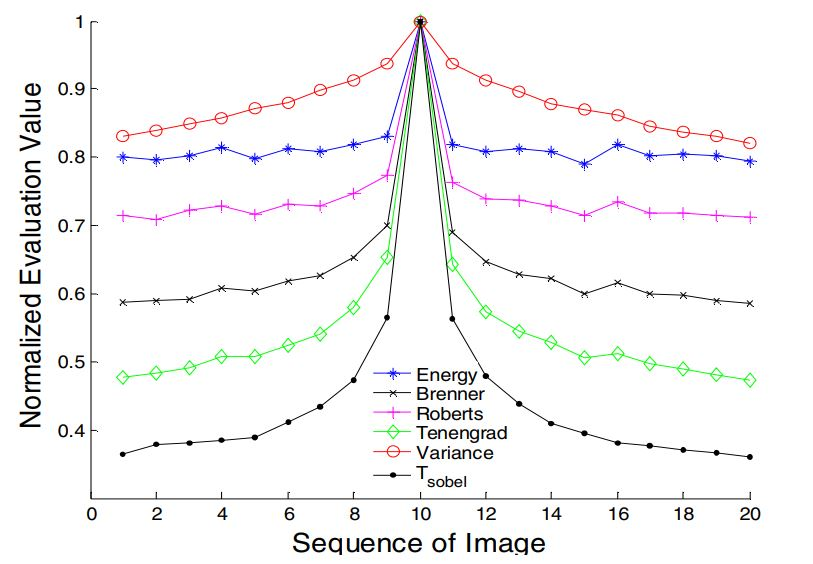
\includegraphics[width=\textwidth]{GraficosEdArt/FocusingWithNoise-mo2012.jpg}
\caption{Resultados de gradiente máximo en imágenes con ruido \citet{Mo2012}}
\label{FocusingWithNoise_mo2012}
\end{figure}

\begin{figure}
\centering
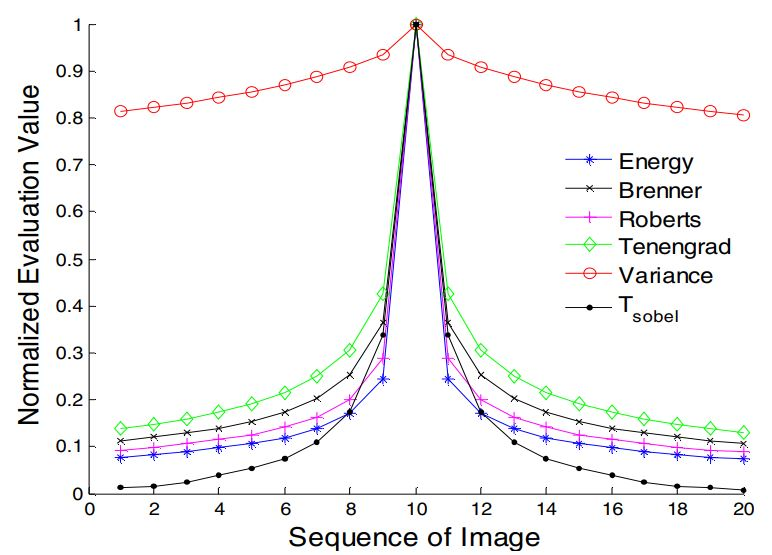
\includegraphics[width=\textwidth]{GraficosEdArt/FocusingWithoutNoise-mo2012.JPG}
\caption{Resultados de gradiente máximo en imágenes sin ruido \citet{Mo2012}}
\label{FocusingWithoutNoise_mo2012}
\end{figure}

\begin{table}[t]
\begin{center}
\begin{tabular}{| c | c | c | c |}
\hline
Función & Gradiente de Energía & Gradiente de Roberts & Gradiente de Brenner\\ \hline
Tiempo & $78.45$ ms & $73.95$ms& $70.05$ ms \\\hline
Función &de Tenengrad & de Varianza & $T_{sobel}$ \\\hline
Tiempo & $82.85$ ms & $184.13$ ms& $30.06$ ms \\ \hline
\end{tabular}
\caption{Comparativa de tiempos entre funciones de gradiente. \citet{Mo2012}}
\label{tab:gradMax}
\end{center}
\end{table} 

Lograr obtener una métrica es un gran paso para poder llevar a cabo este trabajo, sin embargo, la necesidad de poder realizar de manera automática este proceso, requiere otro método de apoyo, para ello en \citet{Zhang:14}  se muestra un método para llevar a cabo el proceso de obtener el enfoque de manera automática, rápida y precisa. \\
\\
El artículo presenta dos métodos de autoenfoque pasivos, el primero lo hace a través de la cantidad de enfoque (DFF) y el segundo con la cantidad de desenfoque (DFD), cada uno de los métodos tiene características, donde el autor propone una versión mejorada del método DFD obteniendo como resultado un método robusto, eficiente y preciso.

\begin{figure}[ht]
\centering
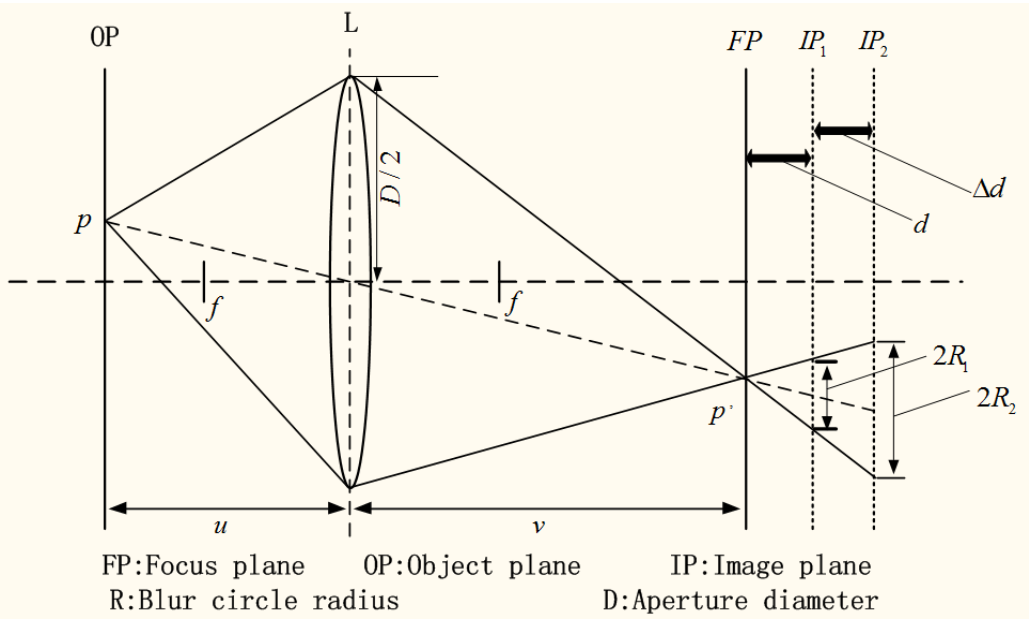
\includegraphics[scale=0.50]{GraficosEdArt/ImagenLentesDFD.PNG} 
\caption{Modelo óptico para formación de imágenes \citet{Zhang:14}}
\label{fig3}
\end{figure}

En la figura \ref{fig3} se muestra al plano focal $FP$,el plano de objeto $OP$  , el plano de imagen uno $IP_{1}$ y el plano de imagen dos $IP_{2}$. La finalidad del método DFD es la estimación de la $d$ y $\Delta d$ como una cantidad de desenfoque con respecto al plano focal, para ello se requieren dos imágenes desenfocadas, de tal forma que se proponen dos alternativas para poder obtenerlas, una es a través del cambio de la distancia de imagen  y la otra a través del cambio de distancia de objeto, el cual se utilizará para este trabajo de investigación.

El método DFF incluye dos fases, la primera se basa en determinar la función de enfoque que describe el grado de borrosidad en diferentes posiciones y la segunda es la búsqueda de la mejor posición de acuerdo a la función de enfoque. Originalmente éste método resulta ser bastante preciso pero costoso, por ello el autor fusiona el método DFF y el DFD mejorado, con la intención de tener uno con una buena mejora.
\\
\begin{figure}[ht]
\centering
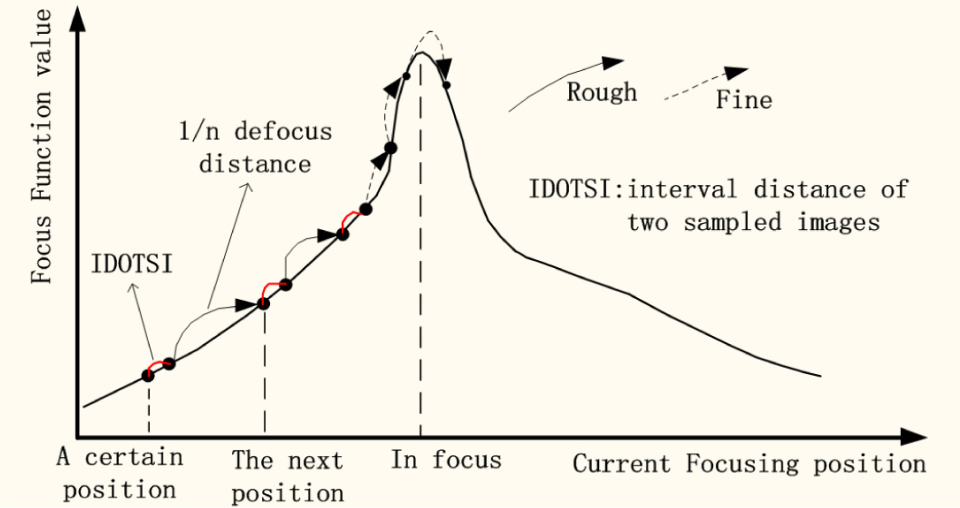
\includegraphics[scale=0.50]{GraficosEdArt/FocusFunctionValue.PNG} 
\caption{Combinación de DFF y DFD mejorado \citet{Zhang:14}}
\label{fig4}
\end{figure}
\\
En la figura \ref{fig4} se muestra la combinación DFF y DFD mejorado, está dividida en dos fases, una fase robusta y otra fina. En la fase robusta se lleva a cabo a través del método DFD mejorado, donde dada dos imágenes se calcula la distancia de desenfoque a un cierto paso, hasta que esta distancia sea más pequeña que cierto valor de umbral, entonces se procede a la fase “fina”, donde se hace uso del método DFF con la búsqueda de la posición del pico de la función (el máximo) a un paso ajustado, lo cual es un paso menor a la profundidad de enfoque. La posición del pico en la función de enfoque corresponde a la posición de enfoque.

Otros modelos que hacen uso de otro tipo de geometría basada en la óptica de los rayos de luz, es el método propuesto por \citet{Subbarao1993} que hace uso de la función de dispersión de punto (PFS) como medio para poder modelar el desenfoque en una imagen. En este artículo el autor utiliza técnicas que no requieren una calibración de cámara , pero sí una búsqueda de parámetros de cámara en el espacio. 

Entre los parámetros a ser utilizados para la implementación de este método se encuentra la distancia focal $f$, la distancia $s$ entre el segundo plano principal y el detector de imagen, y por último el diametro de apertura $D$, en conjunto conforman los parámetros de la cámara, denotados como \textbf{e}.


Este vector de configuración \textbf{e} es usado para poder hallar la función de transferencia óptica la cual hace uso de la función de dispersión de punto, en \citet{Subbarao1993} hace uso de dos modelos \emph{PSF}, el modelo del disco circular y el Gaussiano, en el cuadro \ref{tablaPSF} se muestran las representaciones explícitas de los modelos en su versión algebráica.
Las funciones \emph{OTF} se encuentran en el dominio de las frecuencias, por lo tanto $\omega$, $v$ y $\rho$ son frecuencias espaciales en radianes por unidad de distancia, $J_1$ es la función de Bessel de primer orden.

La función $\rho$ es definida como $\rho(\omega,v) = \sqrt{(\omega ^2 + v^2 )}$ , en $h_b$ $r$ se define como el parámetro de dispersión correspondiente a la desviación estándar, para fines prácticos $r$ es proporcional a $R$, por lo tanto $r = cR$ para una $c < 0$, donde $c$ es constante.




El autor propone tres medidas de enfoque que pueden ser calculadas de manera eficiente bajo un dominio espacial. Entre ellas se encuentra la energía de la imagen ($M_1$), la energía del gradiente de imagen ($M_2$) y la energía del laplaciano de imagen ($M_3$).

La metodología llevada a cabo consta de una primera etapa donde a partir de una imagen ubicada en el plano se genera una secuencia de imágenes con diferente profundidad de campo, de allí que se haga uso de la función de dispersión de punto ($PSF$) y el vector de configuración \textbf{e}, dando como resultado un conjunto de imágenes, donde cada una contiene niveles de borrosidad diferente. Dichas imágenes serán procesadas en cada una de las medidas de enfoque para cada una de las funciones de dispersión de punto, dando lugar a las métricas préviamente mencionadas (con secuencia de imágenes $G_i$) y a las relacionadas con la función $h_b$ cuya $G_i'$ se obtiene a partir de la convolución de una Guassiana bi-dimensional y la imagen, posteriormente se procede a calcular las medidas de enfoque mencionadas con anteriorioridad y así obtener $M_1'$, $M_2'$ y $M_3'$ que representan las medidas de enfoque provenientes de aplicar un filtro pasa-bajas a las imágenes.


Entre los experimentos realizados por el autor, se llevó a cabo sobre tres imágenes ubicadas en el plano (figura \ref{f:objetosSubbarao}), a partir de cada una de ellas se generó una secuencia de imágenes. 

\begin{figure}
 \centering
  \subfloat[\label{f:obj1}]{
    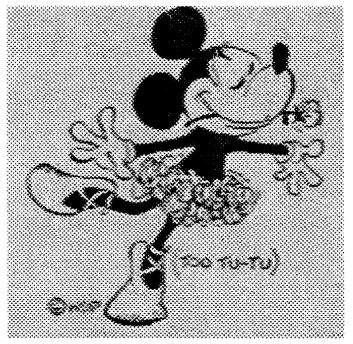
\includegraphics[width=0.3\textwidth]{GraficosEdArt/subobj1.JPG}
    }
  \subfloat [\label{f:obj2}]{
    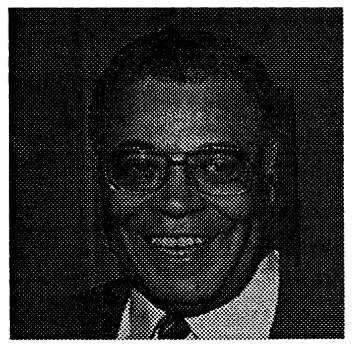
\includegraphics[width=0.3\textwidth]{GraficosEdArt/subobj2.JPG}}
  \subfloat [\label{f:obj3}] {
    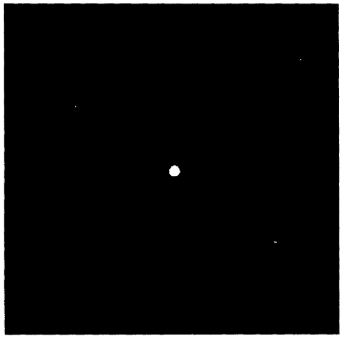
\includegraphics[width=0.3\textwidth]{GraficosEdArt/subobj3.JPG}}
 \caption{Objetos utilizados en experimentos \citet{Subbarao1993}.}
 \label{f:objetosSubbarao}
\end{figure}

Para poder capturar las imágenes se utilizó un sistema de cámaras SPARCS donde se capturaron 97 cuadros, cada uno con diferentes configuraciones, con la finalidad de obtener diferentes cuadros enfocados. El objeto 3 (figura \ref{f:obj3}) tiene altas frecuencias espaciales, este fue elegido para observar los efectos de onda producidos por las medidas de enfoque. La iluminación para los primeros dos objetos (figuras \ref{f:obj1} y \ref{f:obj2}) fue alrededor de 500 1x.\\
\\
Cada objeto fue colocado en diferentes distancias (La figura \ref{f:obj1} a 820 mm, figura \ref{f:obj2} a 950 mm y la figura \ref{f:obj3} a 1320 mm) enfrente de la cámara, de tal manera que se generaron los 97 cuadros con diferente posición de lente y con tamaño de 64 por 64 pixeles. Se midió la profundidad de campo con cada una de las medidas de enfoque, generando las gráficas mostradas en la figura \ref{subaraoSalidas}.


\begin{figure}
 \centering
  \subfloat[\label{obj1:plot}]{
    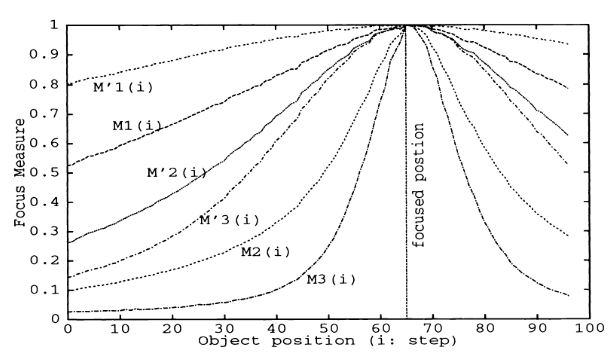
\includegraphics[width=0.7\columnwidth]{GraficosEdArt/objeto1_focusmeasure.JPG}}
    \hfill
  \subfloat[\label{obj2:plot}]{
    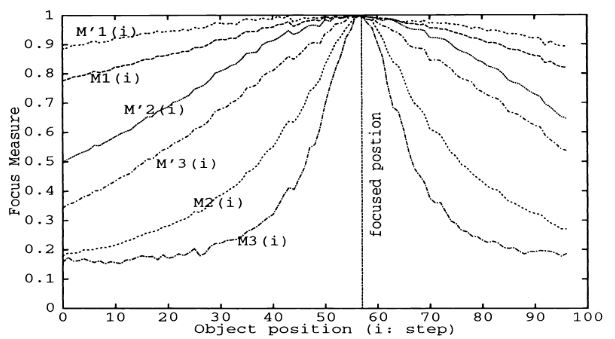
\includegraphics[width=0.7\columnwidth]{GraficosEdArt/objeto2_focusmeasure.JPG}}
    \hfill
  \subfloat [\label{obj3:plot}]{
    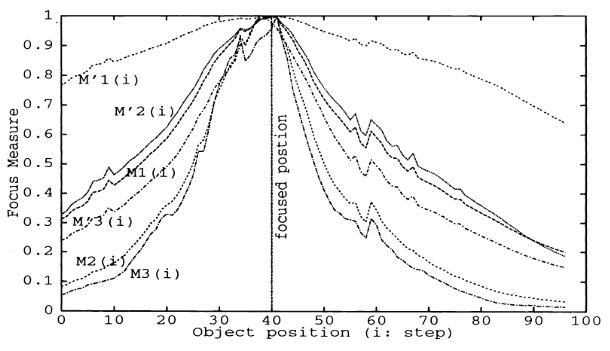
\includegraphics[width=0.7\columnwidth]{GraficosEdArt/objeto3_focusmeasure.JPG}}
 \caption{Curvas de enfoque normalizadas para los objetos 1, 2 y 3 \citet{Subbarao1993}.}
 \label{subaraoSalidas}
\end{figure}




En la figura \ref{subaraoSalidas}  las medidas de enfoque se encuentran normalizadas con respecto a su valor máximo con la finalidad de alcanzar el valor pico en la misma posición.
\\

Para cada una de las métricas se procedió a calcular un porcentaje de cambio en las medidas de enfoque, lo cual es muy útil en la determinación de la dirección de desplazamiento del lente para poder obtener la mejor imagen enfocada. En la ecuación \ref{eqn:percentChange}, $M(i)$ representa la medida de enfoque.

\begin{equation} \label{eqn:percentChange}
\large \% change = \frac{M(i+step - M(i))}{\frac{1}{2}[M(i+step)+M(i)]}
\end{equation}

Entre los criterios utilizados para poder evaluar la mejor medida de enfoque está la monotonicidad, la magnitud de inclinación y la suavidad. Estos criterios son importantes cuando las imágenes estan áltamente borrosas y cuando son enfocadas en su mayoría. Dichas condiciones hacen que las métricas sean complétamente aplicables. 

Las medidas de enfoque $M_1(i)$ y $M_1'(i)$ son suaves, pero la inclinación de la onda se encuentra muy poco prolongada, lo cual la diferencia entre imágenes borrosas y enfocadas es muy pequeña. Por otro lado la medida de enfoque $M_2(i)$ y $M_3(i)$ muestran curvas semi-planas y ruidosas para imágenes muy borrosas, las medidas de enfoque $M'_2(i)$ y $M'_3(i)$ aquellas resultaron ser generalmente suaves y monotonicas, también muestran alta inclinación de las ondas para imágenes borrosas y casi para las enfocadas, sus picos son rasonalmente agudos. Estas dos últimas métricas resultan ser las mejores planteadas por el autor, de tal forma que son buenas opciones para su aplicación en la práctica.

\section{Modelo de formación de imagen.}

%dar una breve intro a lo que viene y mencionar que la mayoría de los términos empleados fueron extraídos del libro de harley



\subsection{El modelo Pin-hole  (homogeneo)}

Previamente se habló del concepto del modelo Pin-hole (modelo de proyección perspectiva), así como también las ecuaciones que lo representan. En este apartado se desarrollara el concepto previamente descrito en la sección~\ref{sec:pin-hole}, llevándolo a cabo en coordenadas homogeneas incorporando ademas al modelo, información de la posición de la cámara en el espacio, con la finalidad de aplicarlo posteriormente en este trabajo de investigación.

\subsubsection{Coordenadas homogeneas \label{coordenadashomogentitle}}

Las coordenadas homogeneas es un instrumento utilizado en la geometría proyectiva para describir un punto en el espacio proyectivo. Dadas unas coordenadas $(x,y)$ en el plano cartesiano, convertirlo en coordenadas homogeneas basta con apilarle una dimensión, quedando como resultado lo descrito en la ecuación \ref{equ:carteToHomogen}. Normalmente las coordenadas homogeneas suelen identificarse como un vector columna, y para un mejor entendimiento en expresiones algebraicas los elementos del vector se suelen poner con letras mayúsculas.

\begin{equation}
    \begin{aligned}
        (x,y) \Rightarrow \left[\begin{array}{c}X\\Y\\1\end{array}\right]
    \end{aligned}
    \label{equ:carteToHomogen}
\end{equation}

En la ecuación \ref{equ:carteToHomogen} se describe un ejemplo de conversión dada una coordenada cartesiana $(x,y)$, el uso de las coordenadas homogeneas facilita el operamiento en geometría proyectiva, ya que como representan vectores columna, pueden ser trabajados con matrices, facilitando las operaciones entre ellas.

En el caso de una coordenada cartesiana de tres dimensiones, el proceso es el análogo.

\begin{equation}
    \begin{aligned}
        (x,y,z) \Rightarrow \left[\begin{array}{c}X\\Y\\Z\\W\end{array}\right]
    \end{aligned}
    \label{equ:carteToHomogen2}
\end{equation}

En la ecuación \ref{equ:carteToHomogen2} se presenta un caso general donde usualmente $W=1$.



\subsubsection{Puntos y líneas en ecuaciones homégeneas}


La representación de una linea bidimensional en un plano es $ax+by+c=0$, donde $a$, $b$ y $c$ son los parámetros de la linea mientras que $x$ y $y$ son las coordenadas cartesianas en el plano. Como lo indica~\cite{hartley_zisserman_2004}, la representación natural de una linea sería el vector $(a,b,c)^\top$. 
Las correspondencias entre líneas y vectores no son perfectamente definidas, ya que no existe una relación uno a uno entre vectores y líneas. Esto se puede verificar, si se tiene una línea recta con ecuación $ax+by+c=0$ se sabe que si se tiene un escalar $k$ diferente de cero, entonces $(ka)x + (kb)y + (kc) = 0$ representa a la misma línea, por otra parte con los vectores, dado $(a,b,c)^\top$ y $k(a,b,c)^\top$ representan la misma línea, solo que se encuentran escalados, pero en principio son equivalentes.

Dado lo explicado con anterioridad, surge un nuevo conjunto llamado \emph{conjunto clase de equivalencia} donde los vectores que lo conforman son vectores \emph{homogéneos} de la forma  $(a,b,c)^\top$ y este conjunto en $\mathbb{R}^3$  forman el espacio proyectivo $\mathbb{P}^2$ donde el vector $(0,0,0)^\top$ es excluido.
\\
Si se tiene un punto con coordenadas $(x,y)$ y si se quisiera encontrar la línea  que yace en este punto, entonces se debe cumplir que $ax+by+c=0$, donde otra forma de denotarlo es através del producto punto y como ya se vió la línea $ax+by+c=0$ se puede escribir como el vector columna $(a,b,c)^\top$ y por otra parte las coordenadas $(x,y)$ en su versión homogénea $(x,y,1)$ como se vió en el apartado \ref{coordenadashomogentitle} que basta con apilarle una coordenada más. Los puntos entonces, como vectores homogéneos son elementos del espacio proyectivo $P^2$.

Visto lo anterior se establece lo siguiente:

\begin{itemize}
    \item El punto \textbf{x} yace en una línea \textbf{l} si y solo si $\textbf{x}^\top \textbf{l} = 0$.
    
    \item La intersección de dos líneas $\textbf{l}$ y $\textbf{l'}$ es el punto \textbf{x} $= \textbf{l} \times \textbf{l'}$
\end{itemize}

Explicado los conceptos anteriores se procede aterrizarlos a lo que se compete, se trata del modelo \emph{pin-hole} explicado con ecuaciones homogeneas, lo cual será de utilidad al momento de realizar las homografías entre imágenes, ya que la mayoría de la teoría se sustenta con este modelo.

\begin{figure}
\centering
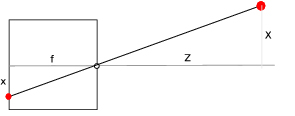
\includegraphics[width=\textwidth]{GraficosEdArt/pinholecameramodel.jpg}
\caption{Modelo de cámara oscura o \emph{pin-hole}.}
\label{pinhole_diagram}
\end{figure}

En la figura \ref{pinhole_diagram} tenemos $f$ que representa la distancia focal, el eje $\mathbb{Z}$ que es el eje perpendicular al plano del orificio, $X$ y $Y$ que son las coordenadas en la espacio y $(x,y)$ son las coordenadas en el plano de la imagen.

Teniendo $(X,Y,Z)$ como coordenadas conocidas de un punto $P$, entonces es posible calcular las coordenadas de $(x,y)$ del punto $P'$ proyectado en el plano de imagen $I$.

\begin{equation}
    \label{proyeccionEqu}
     x = -f\frac{X}{Z} \hspace{1cm}  y = -f \frac{Y}{Z}  
\end{equation}

Como usamos coordenadas homogeneas, podemos multiplicar cualquier coordenada por una constante diferente a cero. como se puede ver en la ecuación~\ref{proyeccionEqu}, las coordenadas tienen un signo negativo, pues planteamos que el plano de proyeccion esta situado a una distancia $f$ del origen del sistema. Sin embargo podemos ubicar el plano de proyección a una distancia $f$ enfrente del origen del sistema, lo cual es equivalente a multiplicar cada coordenada homogenea por $-1$., y así obtenemos las siguientes ecuaciónes:

\begin{equation}
     x = f\frac{X}{Z} \hspace{1cm}  y = f \frac{Y}{Z}
     \label{proyeccionEqu2}
\end{equation}

Partiendo de esto se procede a transformarlo en a coordenadas homogéneas, como sigue:
\begin{equation}
\begin{aligned}
\lambda\left[\begin{array}{cc}x\\y\\1\end{array}\right]
 & = & \left[\begin{array}{cccc}
f & 0 & 0 & 0\\
0 & f & 0 & 0\\
0 & 0 & 1 & 0
\end{array}\right]
\left[\begin{array}{c}X\\Y\\Z\\1\end{array}\right]
\end{aligned}
\label{eq:ProyMatrix}
\end{equation}
donde $\lambda$ es un escalar diferente de cero.

La ecuación de arriba es el modelo geométrico: $(X,Y,Z)^\top$ y $(x,y)^\top$ son las coordenadas en el espacio y en el plano de la imagen, $f$ la distancia focal medida en metros o milímetros. En la práctica las coordenadas de la cámara son medidas en pixeles.

Para convertrir las distancias en pixeles se introducen los escalares $s_x$ y $s_y$, como sigue:

\begin{equation}
\begin{aligned}
\lambda\left[\begin{array}{cc}x\\y\\1\end{array}\right]
 & = & \left[\begin{array}{cccc}
s_xf & 0 & 0 & 0\\
0 & s_yf & 0 & 0\\
0 & 0 & 1 & 0
\end{array}\right]
\left[\begin{array}{c}X\\Y\\Z\\1\end{array}\right]
\end{aligned}
\label{eq:ProyMatrix_2}
\end{equation}

Se puede notar que las coordenadas $(x,y)$ son medidas en pixeles, por lo tanto se puede realizar lo siguiente.

\begin{equation}
    f_x=s_x f \hspace{1cm} f_y = s_y f
\end{equation}

Dando como resultado lo siguiente:

\begin{equation}
\begin{aligned}
\lambda\left[\begin{array}{cc}x\\y\\1\end{array}\right]
 & = & \left[\begin{array}{cccc}
f_x & 0 & 0 & 0\\
0 & f_y & 0 & 0\\
0 & 0 & 1 & 0
\end{array}\right]
\left[\begin{array}{c}X\\Y\\Z\\1\end{array}\right]
\end{aligned}
\label{eq:ProyMatrix_3}
\end{equation}  

Las coordenadas del pixel no están dados con respecto a un cuadro que es centrado en el eje óptico, en lugar de eso, las coordenadas están en el cuadrante positivo. Esto implica una traslación de las coordenadas del cuadro, que se incluye:

\begin{equation}
\begin{aligned}
\lambda\left[\begin{array}{cc}x\\y\\1\end{array}\right]
 & = & \left[\begin{array}{cccc}
f_x & 0 & u_0 & 0\\
0 & f_y & v_0 & 0\\
0 & 0 & 1 & 0
\end{array}\right]
\left[\begin{array}{c}X\\Y\\Z\\1\end{array}\right]
\end{aligned}
\label{eq:ProyMatrix_4}
\end{equation}  

Por último, se requiere añadir el factor de sesgo $\alpha$ que nos dice que tanto varía la cizalladura en el sistema. Dado aquello obtenemos el modelo interno de la cámara mostrado en la figura \ref{eq:ProyMatrix_5}, donde la matriz $K$ contiene los parámetros internos de la cámara.


\begin{equation}
\begin{aligned}
\lambda\left[\begin{array}{cc}x\\y\\1\end{array}\right]
 & = & K
\left[\begin{array}{c}X\\Y\\Z\\1\end{array}\right]
\end{aligned}
\label{eq:ProyMatrix_5}
\end{equation}  
 
\begin{equation}
\begin{aligned}
\lambda\left[\begin{array}{cc}x\\y\\1\end{array}\right]
 & = & \blk{K} &\left[\begin{array}{cc} \blk{R} & \blk{T}\\\blk{0} & 1\end{array}\right]
\left[\begin{array}{c}X\\Y\\Z\\1\end{array}\right]
\end{aligned}
\label{eq:ProyMatrix_6}
\end{equation}  

En la ecuación \ref{eq:ProyMatrix_6} se tiene un caso cuando la cámara no se encuentra en el origen, R es una matriz de 3x3 que representa la orientación de la cámara, y T es el vector que representa la translación de la cámara, esto es la posición de la cámara con respecto al marco de referencia (La cámara está en el origen cuando R es la identidad y T es un vector de ceros).

 \begin{figure}[h]
\centering
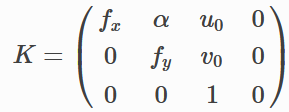
\includegraphics[scale=0.7]{GraficosEdArt/pinholeHomogenea_6.PNG}
\caption{Matriz de parámetros internos de la cámara.}
\label{kmatrix}
\end{figure}  
 
\subsection{Puntos de fuga.}


Una de las características distintivas de la perspectiva de proyección es, dada una imagen de un objeto que se extiende hasta el infinito puede tener una extensión finita. Por ejemplo, como se muestra en la figura \ref{demoVanishingPoint}, las rieles se extienden al infinito, pero, existe un punto que se mantiene fijo e inmovible, conocido como el punto de fuga.

 \begin{figure}[h]
\centering
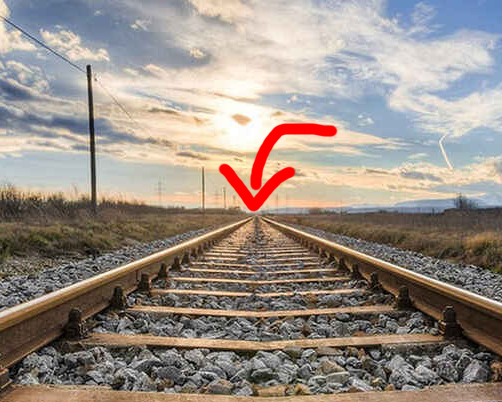
\includegraphics[scale=0.5]{GraficosEdArt/puntoFugaDemo.jpg}
\caption{La marca roja indica la zona donde el punto de fuga se encuentra.}
\label{demoVanishingPoint}
\end{figure}  

En la figura \ref{fig:vanishinPointGeo} se observa una línea que converge a una coordenada $\mathcal{v}$ en la imagen. A esa coordenada se le conoce como el punto de fuga. Cualquier linea en el espacio es paralela a una linea con la misma orientación pero que pasa por el centro de proyección de la cámara; el punto en la imagen donde todas las lineas paralelas a esa  linea convergen corresponde a la intersección de la linea que pasa por el origen con el plano de la imagen. Una linea  que pasa por centro de la cámara se puede representar con un vector unitario en $\mathcal{R}^3$.

 \begin{figure}[h]
\centering
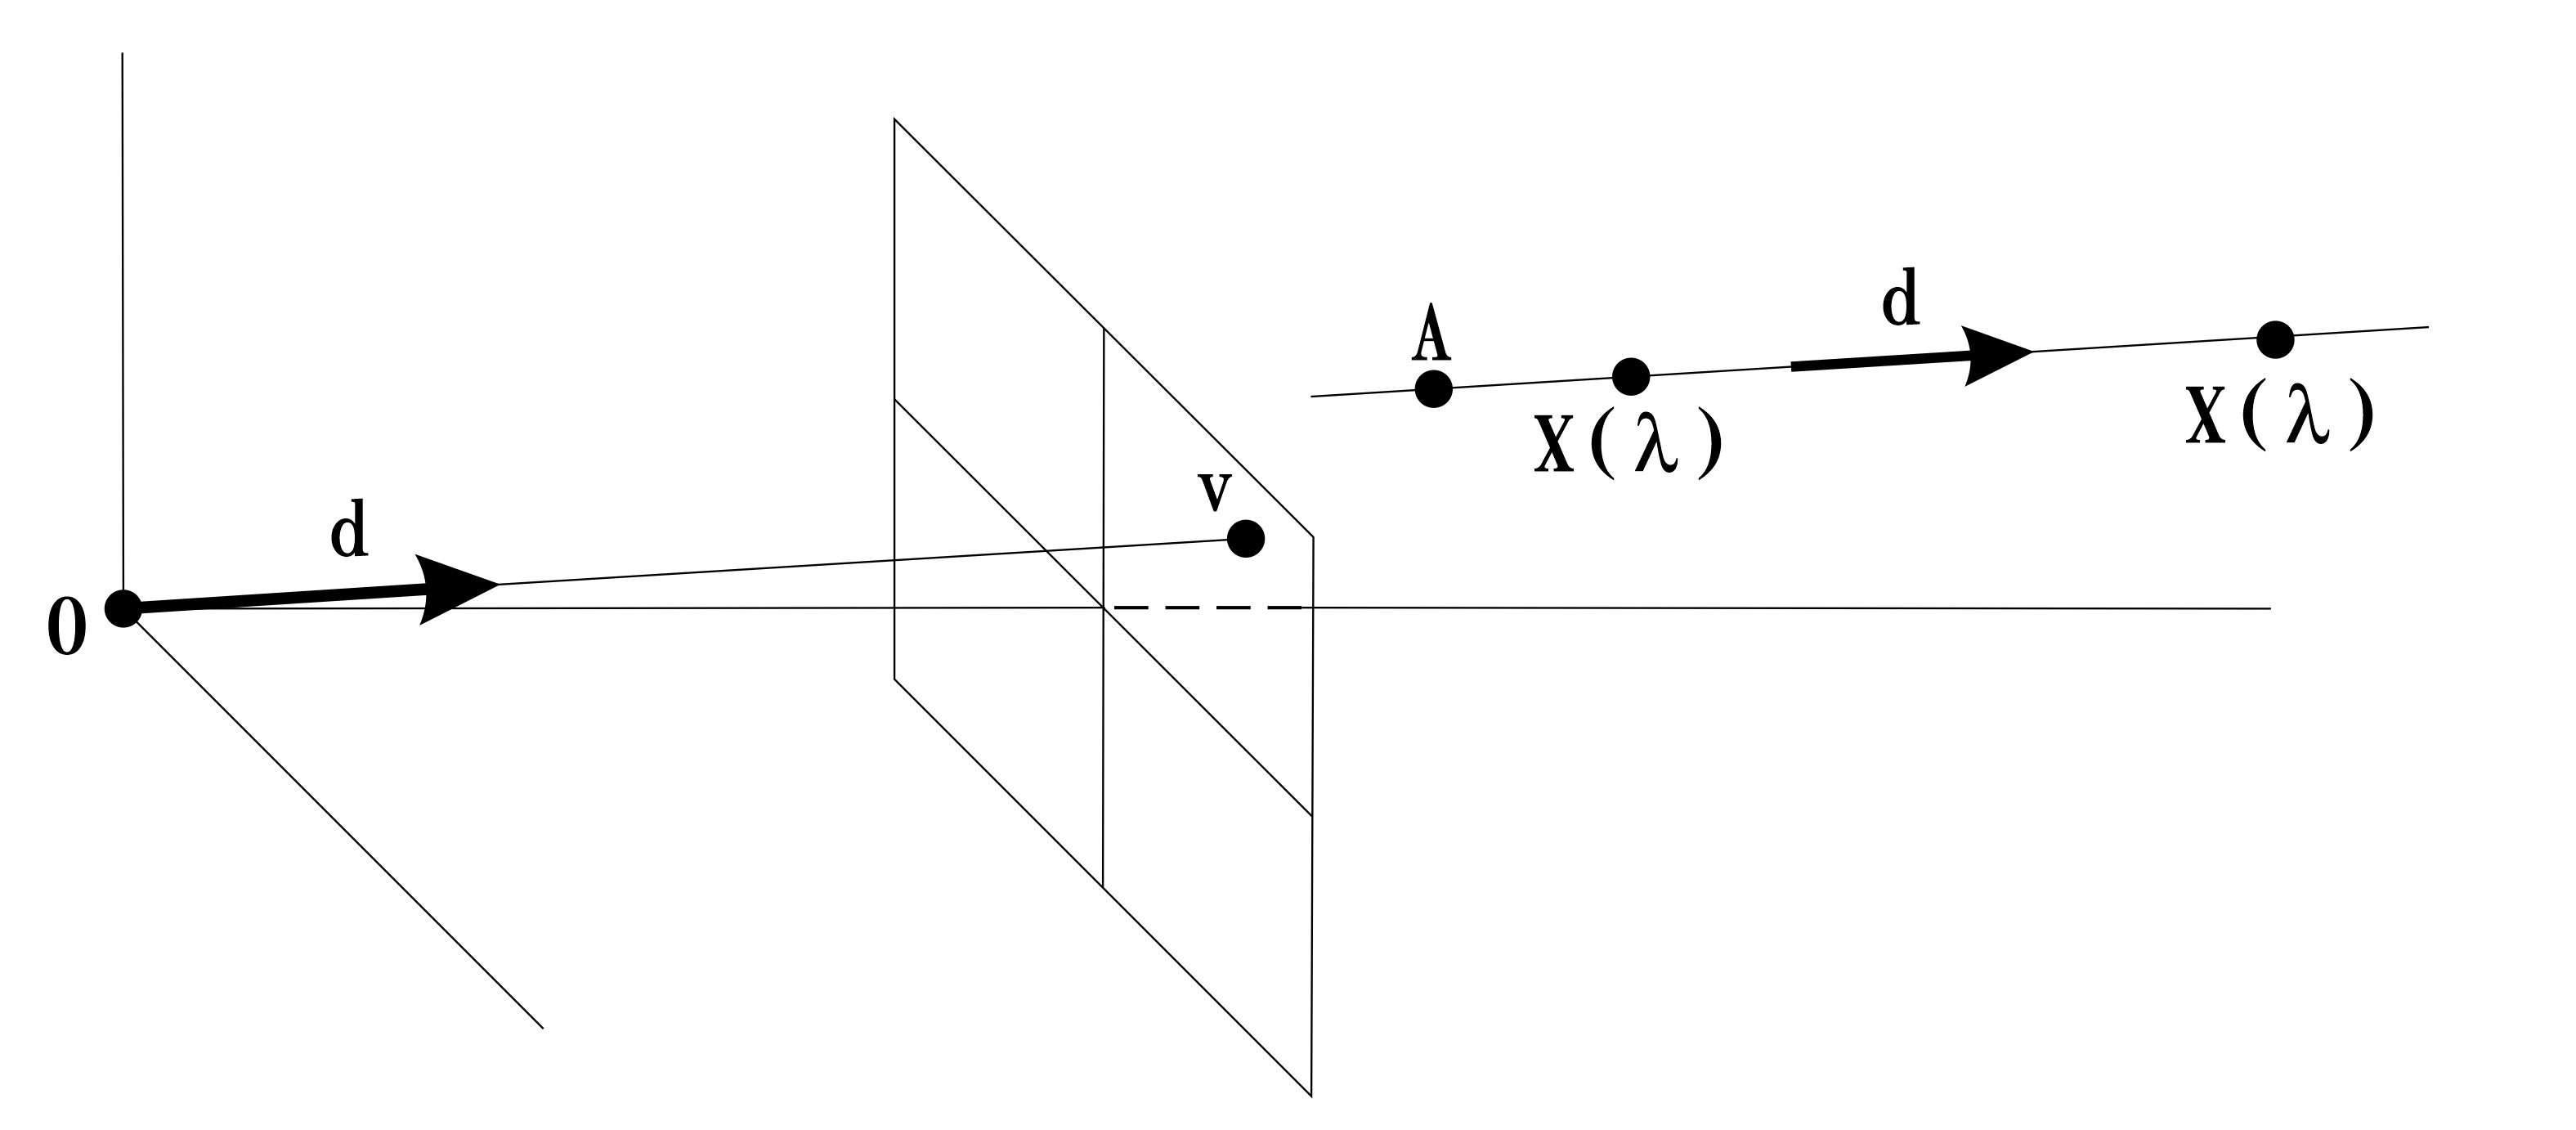
\includegraphics[scale=0.5]{GraficosEdArt/Figura_8-14_Harley.png}
\caption{Geometría del punto de fuga.}
\label{fig:vanishinPointGeo}
\end{figure}  


En la figura \ref{fig:paralelasPuntoFuga} se muestra un ejemplo del comportamiento de los rayos paralelos que inciden en el plano de imagen, se establecen dos conjuntos de líneas paralelas cuya convergencia se da en el punto de fuga.

 \begin{figure}[h]
\centering
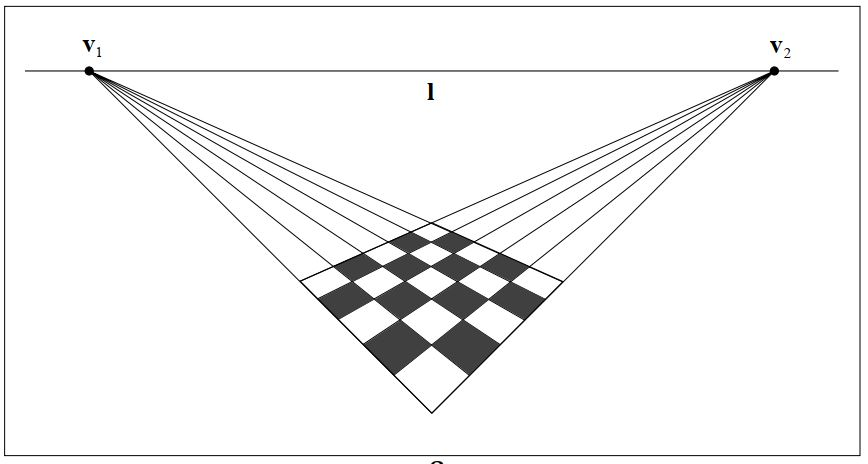
\includegraphics[scale=0.5]{GraficosEdArt/vanishinpointlines.JPG}
\caption{Conjuntos de líneas paralelas que convergen en los puntos de fuga $v_1$ y $v_2$.\citet{hartley_zisserman_2004}}
\label{fig:paralelasPuntoFuga}
\end{figure}  

Teniendo en cuenta el contexto de que sí se tiene una cámara que se aproxima hacia algún objeto, el marco de referencia sería el mismo si el objeto se moviera hacia la cámara, y de allí que el punto de fuga se mantenga en el mismo lugar dado que el objeto se desplaze hacia la cámara. Por lo tanto el punto de fuga resulta ser una herramienta útil para llevar a cabo este trabajo de investigación. 

\subsection{Homografia.}



En este apartado se menciona lo referente a dar solución al problema de la estimación, a través del uso de homografías, definido como un mapeo invertible a patir de un plano $\mathbb{P}^2$ a él mismo, tal que tres puntos son colineals \footnote{Esto es, que yacen en la misma línea.} si y solo sí al mapearlos continuan siendo puntos colineales. Una forma simple de entender una homogafría es que es un mapeo de planos, como se muestra en la figura \ref{fig::mapping}, dado un par de imágenes, donde la segunda corresponde con la primera, existe una superficie del plano tal que un punto $\mathbf{x}$ corresponde a $\mathbf{x'}$ dada una traslación y una rotación.
\\
 \begin{figure}[h]
\centering
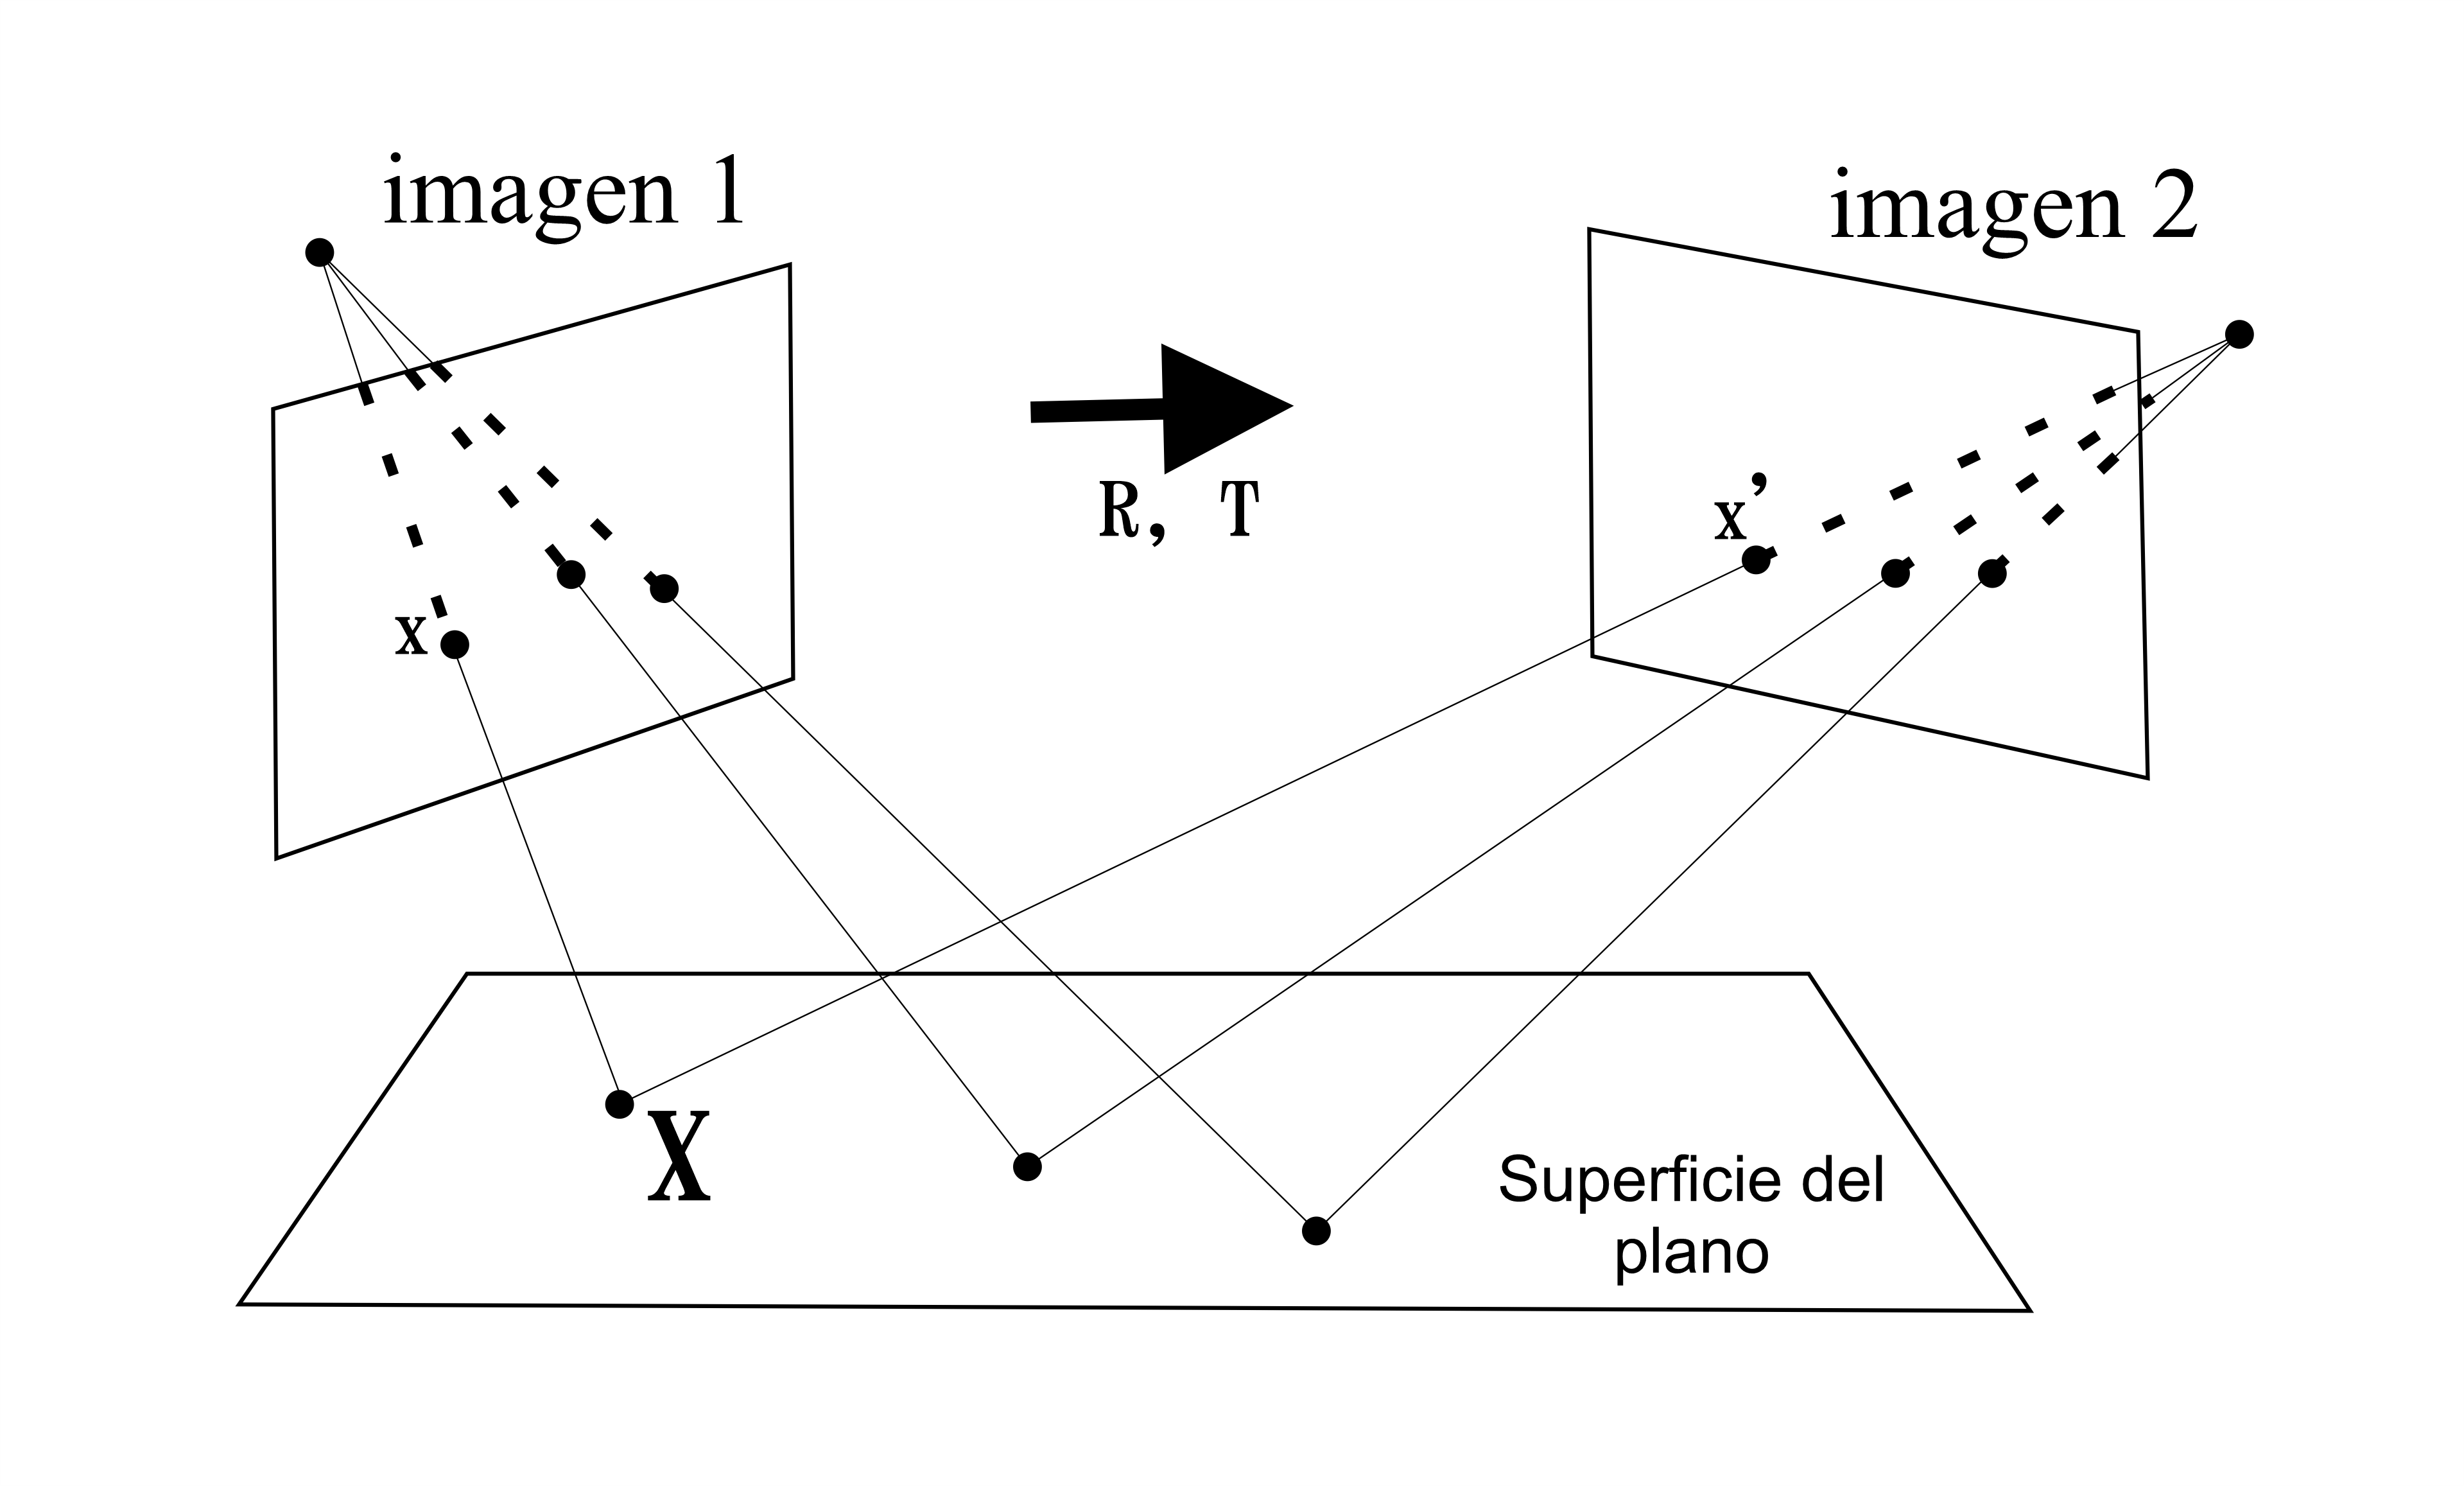
\includegraphics[scale=0.35]{GraficosEdArt/Imagenpag36.png}
\caption{Perspectiva de proyección entre dos planos inducidos por una superficie del plano}
\label{fig::mapping}
\end{figure}  

% Encontrar la homografía asociada a un sistema consiste en 
% hallar la matríz $H$ a partir de un conjunto de 
% correspondencias, de tal forma que ésta da información sobre
% las transformaciones asociadas al objeto $P$ con su 
% respectiva % correspondencia $P'$.

Matemáticamente una homografía se define como sigue:
Se considera un punto $\mathbf{x} = (u,v,1)$ en una imagen con su respectiva correspondencia $\mathbf{x}' = (u',v',1)$. Una homografía es una matríz de 3 por 3, típicamente denotada como $H$.
\begin{equation}
\begin{aligned}
H & = & \left[\begin{array}{ccc}
h_{1,1} & h_{1,2} & h_{1,3} \\
h_{2,1} & h_{2,2} & h_{2,3} \\
h_{3,1} & h_{3,2} & h_{3,3} 
\end{array}\right]
\end{aligned}
\label{eq:homografyMat}
\end{equation}

La relación entre el pixel $\mathbf{x}$ y su correspondiente $\mathbf{x'}$ dada una transformación --ya sea escalamiento, rotación o traslación-- se plantea como sigue.

\begin{equation}
    \mathbf{x}^\prime =\mathbf{H}\mathbf{x}
\end{equation}
Dos imágenes se encuentran relacionadas con una homografía si y solo si ambas imágenes son vistas en el mismo plano pero con diferente transformación, o bien si ambas imágenes son tomadas desde la misma cámara pero de diferente punto de vista.


\subsection{Velocidad de cambios en la imagen a partir de movimiento lineal.}
En este apartado se pretende describir el proceso para poder establecer la homografía asociada al sistema, dado un movimento en cada uno de los objetos segmentados en la imagen. 

Dado un punto en el espacio $\mathbf{P'}$ con coordenadas $(X,Y,Z)$ y su correspondiente $\mathbf{P}$ ubicado en el plano de la imagen con coordenadas $(x,y)$, se forma un caso particular cuando $f = 1$ apartir de la ecuación \ref{proyeccionEqu2} como sigue:

\begin{equation}
    \label{equ::planoSpace}
    \begin{aligned}
        (x,y) = (X/Z, Y/Z)
    \end{aligned}
\end{equation}


Sea $[u,v]^\top$ el vector de flujo óptico \footnote{Es un campo vectorial que representa las variaciones de intensidad encontradas en la imagen producidas por el movimiento relativo entre la cámara y la escena}en la imagen y  $T = [T_x,T_y,T_z]^\top$ el vector de velocidades traslacionales en el espacio. 


En \citet{Ullman1979} describe el comportamiento de una imagen en la retina que se encuentra en movimiento, de tal forma que establece lo siguiente:
\begin{equation}
    \begin{aligned}
        u = u^T + u^R \hspace{1.5cm} v = v^T + u^R
    \end{aligned}
    \label{equ:velRelacionTrasRot}
\end{equation}
\begin{equation}
    \begin{aligned}
        u^T = (-T_x +xT_z)/Z \hspace{1.5cm} v^T = (-T_y+yT_z)/Z 
    \end{aligned}
    \label{equ:velTraslacional}
\end{equation}
\begin{equation}
    \begin{aligned}
        u^R = -B + Cy + Axy \hspace{1.5cm} v^R = -Cx + A + Ay^2 - Bxy 
    \end{aligned}
    \label{equ:velRotacional}
\end{equation}

En la ecuación \ref{equ:velRelacionTrasRot} establece la relación entre la velocidad traslacional $\{u^T,v^T\}$ y rotacional $\{u^R,v^R\}$,  

Considerando el caso particular donde no existen componentes rotacionales $u^R = v^R = 0$, el sistema resultande quedaría de la siguiente manera:

\begin{equation}
    \begin{aligned}
    \left[\begin{array}{c}
u \\
v
\end{array}\right]&=&\frac{1}{Z}&\left[\begin{array}{ccc}
    -1 & 0 & x  \\
     0 &-1 & y
\end{array}\right]&\left[\begin{array}{c}
T_x \\
T_y\\
T_z
\end{array}\right]   
\end{aligned}
\label{equ:flujoOpticoSistema}
\end{equation}

Sea $\vec{x}_H =[x,y,w]^\top$ un vector homogeneo en el plano de la imagen y $\vec{X}_H = [X,Y,Z,W]$ un vector homogeneo en el espacio.

Dada una matriz $K$ que representa la matriz de calibración y una matriz $R$ la matriz de rotación, entonces se establece el siguiente sistema.

\begin{equation}
    \begin{aligned}
    \vec{x}_H&=&K&\left[\begin{array}{cc}
    R,T
\end{array}\right]&\vec{x}_H   
\end{aligned}
\label{equ:Homografia1}
\end{equation}
Considerando el caso donde la matríz de rotacion es igual a la matriz identidad ($R = I$).

\begin{equation*}
    \begin{aligned}
    \vec{x}_H&=&K&\left[\begin{array}{cc}
    I,T
\end{array}\right]&\vec{X}_H   
\end{aligned}
\end{equation*}
\begin{equation*}
    \begin{aligned}
    K^{-1}\phi_H&=&\left[\begin{array}{cc}
    I,T
\end{array}\right]&\vec{X}_H   
\end{aligned}
\end{equation*}

Descomponiendo las ecuaciones previamente descritas de acuerdo a los componentes de cada vector, queda como sigue:

\begin{equation}\label{equ:homografiaH}
    \begin{aligned}
    K^{-1}\vec{x}_H&=&\chi&=&\left[\begin{array}{cccc}
    1&0&0&T_x\\
    0&1&0&T_y\\
    0&0&1&T_z
\end{array}\right]&\left[\begin{array}{c}
     X\\
     Y\\
     Z\\
     W
\end{array}\right]&=&\left[\begin{array}{c}
X+T_xW\\
Y+T_yW\\
Z+T_zW
\end{array}\right]&=&\left[\begin{array}{c}
     x_k\\
     y_k\\
     w_k
\end{array}\right]
\end{aligned}
\end{equation}

En la ecuación \ref{equ:flujoOpticoSistema} se tiene que dado un punto con coordenadas $(x,y)$ en el plano de la imagen, se desplaza en el espacio con una velocidad de traslación $(T_x,T_y,T_z)$. Si se consideran estas velocidades como constantes, el desplazamiento del pixel $(x,y)$ estará dado por $(u\Delta_t,v\Delta_t)$ dando lugar a lo siguiente:

\begin{equation}
\label{equ:stateNext}
    \begin{aligned}
        x+u\Delta t = x'\\
        y+v\Delta t = y'
    \end{aligned}
\end{equation}

\begin{equation}
\label{equ:flowVelocityDeltaT}
    \begin{aligned}
        u\Delta t= \frac{-T_x + xT_z}{Z}\Delta t\\
        v\Delta t = \frac{-T_y + yT_z}{Z}\Delta t
    \end{aligned}
\end{equation}

En la ecuación \ref{equ:stateNext} se establece una estimación entre una posición actual $(x,y)$ tras haberse desplazado. Los valores $(x',y')$ representan el valor estimado de la posición del pixel. En la ecuación \ref{equ:flowVelocityDeltaT} se detalla la relación entre el flujo óptico de las posiciones y las velocidades traslacionales $(T_x,T_y,T_z)$. De aquí es evidente que la ecuación \ref{equ:stateNext} se puede dejar en términos de la ecuación \ref{equ:flowVelocityDeltaT} dando como resultado lo siguiente:


\begin{equation}
    \label{equ:homografiaDesarrollo}
    \begin{aligned}
        \left[\begin{array}{c}
        x'\\
        y' 
    \end{array}\right]&\left[\begin{array}{c}
         X\\
         Y\\
         Z\\
         W
    \end{array}\right]&=&\left[\begin{array}{c}
    X+T_xW\\
    Y+T_yW\\
    Z+T_zW
    \end{array}\right]&=&\left[\begin{array}{c}
         x_k\\
         y_k\\
         w_k
    \end{array}\right]
    \end{aligned}
\end{equation}


\begin{equation}
    \label{equ:homografiaNoHomogen}
    \begin{aligned}
         x'= x+\frac{-T_x + xT_z}{Z}\Delta t\\
         y'= y+\frac{-T_y + yT_z}{Z}\Delta t
    \end{aligned}
\end{equation}

Dejando de forma matricial la ecuación anterior se obtiene la homografía asociada al sistema en coordenadas homogeneas.


\begin{equation}
    \label{equ:homografiaMatricialFinal}
    \begin{aligned}
        \left[\begin{array}{c}
        x'\\
        y'\\
        1
    \end{array}\right]=&\frac{1}{Z}&\left[\begin{array}{ccc}
    q & 0 & -T_x\Delta t\\
    0 & q & -T_y \Delta t\\
    0 & 0 & 1
    \end{array}\right]\left[\begin{array}{c}
         x\\
         y\\
         1
    \end{array}\right]
    \end{aligned}
    \hspace{2pt}
    q = z + T_z \Delta t
\end{equation}
%Por ser una relación homogenea al multiplicarlo por un escalar diferente de cero sigue siendo el mismo objeto.
%Poner forma matricial de la homografía para que sea más evidente.

\section{Seguimiento de objetos en la imagen}

Otro concepto muy importante es lo referente al tema de seguimiento, que se trata de un problema común y muy demandado en cuanto a sistemas militares, video-vigilancia, detección de señales de tránsito, entre otras. El seguimiento múltiple de objetos da lugar a poder manipular diferentes objetos en la escena, y asignar un identificador a cada uno con la finalidad de poder extraer información requerida (posición, caracterísicas, descriptores).

En el capítulo 4 de \citet{Waltz2008} se presentan diferentes algoritmos relacionados con el seguimiento de objetos múltiple, donde en el presente trabajo de investigación se hablará en particular del algoritmo de búsqueda del vecino más cercano que es sencillo de aplicar cuando los objetos a seguir son representados por puntos.

Jeffrey K. Uhlmann menciona que la idea del algoritmo es estimar cada posición del objeto en el instante de que se registre una nueva posición, y entonces asignarle aquel reporte al objeto más cercano a tal estimación.

\subsection{La regla del vecino más cercano}

En \citet{T.M.COVER2012} define a la regla del vecino más cercano como un conjunto de $n$ pares,tal que cada tupla conformada por  $(x_1,\theta_2),\cdots ,(x_n,\theta_n)$ y que los valores de $x_i's$ toman valores en un espacio $\mathbb{X}$ sobre el cual está definida una métrica $d$ y los $\theta_i's$ toman valores en el conjunto $\{1,2, \cdots  ,M\}$ donde $M$ representa total de clases. Cada $\theta$ es considerada a ser el índice de la categoría por el cual el i-ésimo dato pertenece, así se puede decir que el $x_i$ pertenece a $\theta_i$.\\
Dado un dato $x_n' \in \{x_1, x_2, \cdots, x_n\}$ es un vecino más cercano a $x$ si
\begin{equation}
    \begin{aligned}
        \min{d(x_i,x)} = d(x_n',x) \hspace{2pt} i=1,2,\cdots,n.
    \end{aligned}
    \label{eqn:NNRULE}
\end{equation}

En la ecuación \ref{eqn:NNRULE} se compara un par de datos $(x,x')$, si la distancia entre ellos es la menor absoluta, entonces $x'$ pertenece a la clase $\theta$ de $x$. Esto abre la posibilidad de realizar un seguimiento múltiple de objetos en un cuadro de video, de tal forma que cada objeto es seguido de acuerdo a la regla del vecino más cercano, independientemente de la cantidad de objetos.

